\section{Evaluating GAN performance}
Evaluating performance of a discriminative model is a rather straightforward issue. One would reserve a portion of data available for a test data set and after training run the model on this data set and count the number of samples correctly classified. With generative models things get more complicated. Judging the quality of generated samples, whether these are images, text or something else, can be challenging and often subjective. However, this has to be done in order to compare different GANs regularly proposed by researches and therefore some creative ideas were proposed to tackle this problem. Some of the methods can be applied only in a particular domain, like generating images displaying multiple objects, while others can be applied to an arbitrary GAN. 
\subsection{Manual evaluation}
The best way to judge the quality of generated contend is still by using real people. For example, Ian Goodfellow \textit{et al.} have created a simple website\footnote{The website can be accessed under  \url{http://infinite-chamber-35121.herokuapp.com/cifar-minibatch/}}, showing user a number of pictures, some of which are generated and some are real. The user is then asked to choose the pictures which he or she thinks were generated by the network. Moreover, the quality of an image is also indicated by the time spent to decide whether is it real or not. Therefore, Emily Denton \textit{et al.} did several test varying the amount of time user was able to see an image before it disappeared~\cite{laplacian_gan}. If the number of positive responses declines with the increase of the amount of time available to judge an image, it is a signal of the poor image quality.
\subsection{Annealed importance sampling (AIS)}
\subsection{Inception score}

\subsection{Generative adversarial metric(GAM)} \label{sec:gam}
Generative adversarial metric (GAM) is an another way of comparing the performance of two GANs. This metric does quantify the quality of a single GAN but rather can give a hint on which of two compared networks performs better. This is done by swapping the GANs' discriminators, as shown in figure 
\begin{figure}[h]
	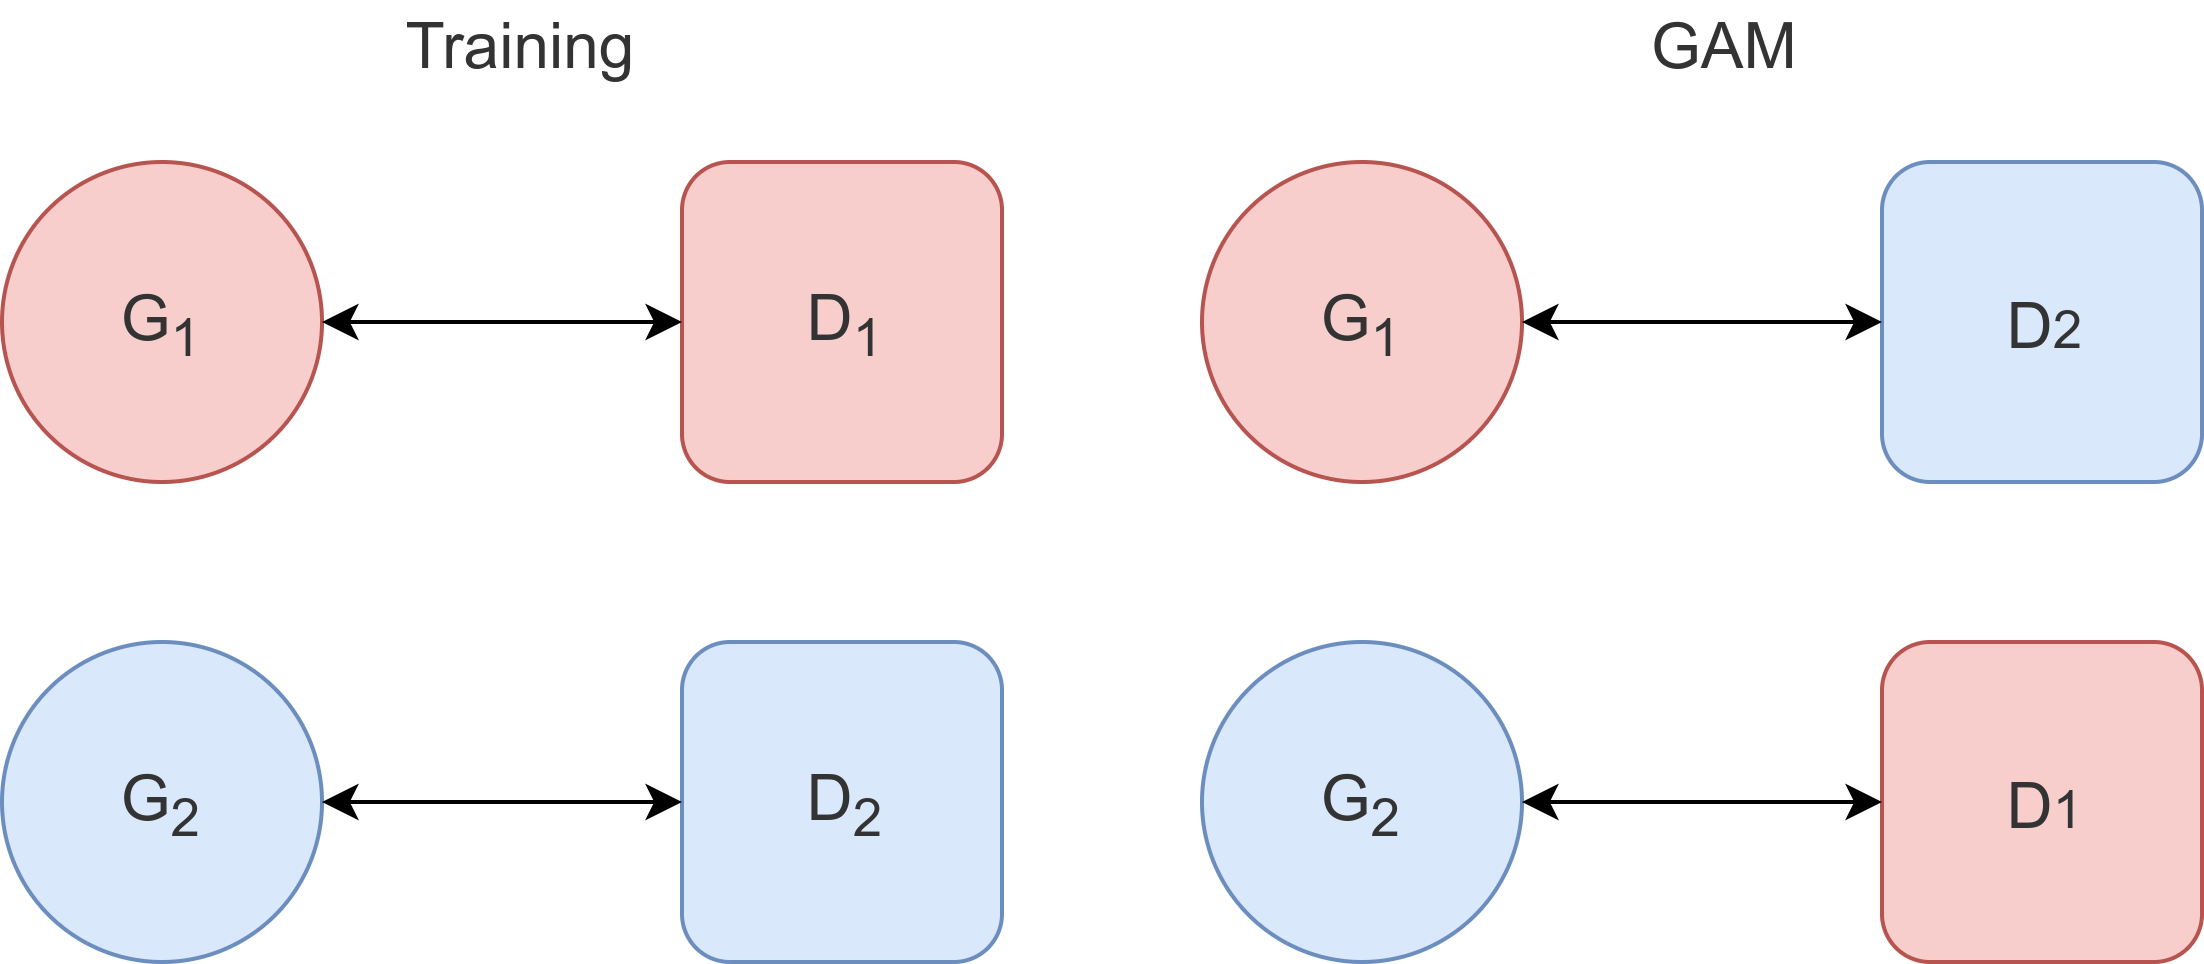
\includegraphics[width=\textwidth]{figures/gam}
	\caption{Visualization the GAM idea. First GAN consists of a generator $G_1$ and a discriminator $D_1$, the second one of $G_2$ and $D_2$ respectively. When the GAM is computed, GANs swap their discriminators, so that $D_1$ judges whether images data produced by $G_2$ look realistic or not, while $D_2$ does the same for $G_1$.}
	\label{fig:gam}
\end{figure}
 
After exchanging discriminators two quantities are computed:
\begin{align} \label{eq:gam_real}
	r_{real} &= \frac{\epsilon(D_1(x_{real}))}{\epsilon(D_2(x_{real}))} \\ 
	r_{generated} &= \frac{\epsilon(D_1(G_2(z)))}{\epsilon(D_2(G_1(z)))}, \label{eq:gam_gen} 
 \end{align}
where $\epsilon(\cdot)$ denotes the misclassification ratio which is be computed by 
\begin{equation*}
	\frac{\text{correctly classified samples}}{\text{total number of samples}}.
\end{equation*} 
Then, depending on the values of the two indicators, we can conclude which GAN performs better:
\begin{equation}
\text{winner} = \begin{cases}
	GAN_1, & \text{if } r_{generator} < 1 \text{ and } r_{real} \approx 1 \\
	GAN_2, & \text{if } r_{generator} > 1 \text{ and } r_{real} \approx 1 \\
	\text{tie}, & \text{if } r_{generator} \approx 1 \text{ and } r_{real} \approx 1  \\
	\text{undefined}, & \text{if } r_{real} \neq 1	
	\end{cases}
\end{equation}
Note that because we actually want to compare the generators, such a comparison is possible only if both discriminators perform equally well, which is indicated by the condition $r_{real} \approx 1$.  
